\chapter{Confronto tra i linguaggi}
\subsection{Sintassi}
Objective-C, in quanto lunguaggio basato su C, ha introdotto nuove parole chiave per differenziare i nuovi tipi da quelli C, utilizzando il simbolo @. Swift, in quanto linguaggio indipendente, non applica alcuna distinzione.\\
Quest'ultimo elimina inoltre alcune delle convenzioni utilizzate nei linguaggi di programmazione più datati: non è necessario utilizzare il punto e virgola per terminare un blocco di codice e non sono necessarie le parentesi per le espressioni condizionali negli statement if/else.\\
Un'altra differenza sostanziale rispetto ad Objective-C è la sintassi usata per le chiamate di funzione: viene utilizzato il punto per identificare la funzione e le virgole per separare gli argomenti della stessa.
\subsection{Manutenzione del codice sorgente}
Objective-C non può evolvere senza attendere l'evoluzione del linguaggio C sottostante; quest'ultimo richiede al programmatore il mantenimento di due files separati per migliorare il tempo di compilazione e l'efficienza di esecuzione, problema che si ripercuote su Obj-C.\\
In Swift questo problema non si presenta ed il compilatore è in grado di riconoscere automaticamente le dipendenze tra i file costituenti di un progetto, utilizzando inoltre il meccanismo di \textit{build} incrementali.
\subsection{Tooling}
I meccanismi ausiliari di aiuto alla programmazione, quali evidenziazione della sintassi ed i suggerimenti di Swift non sono ancora alla pari di quelli Objective-C, fatto che si rende evidente confrontando due files scritti nei due linguaggi all'interno di XCode. Inoltre, gli strumenti di \textit{refactoring} non sono ancora disponibili per Swift.
\subsection{Runtime}
Il runtime di Objective-C è generalmente più robusto e permette meccanismi quali \textit{reflection} e \textit{deep-introspection} di oggetti e tipi, che al momento non sono disponibili in Swift.
\subsection{Sicurezza} 
Un aspetto interessante di Objective-C è il comportamento dei puntatori (in particolare quelli nil). In questo linguaggio non accade nulla se un metodo viene invocato con una variabile puntatore non inizializzata: questa linea di codice viene considerata una non-operazione (no-op). Questo comportamento può avere effetti impredicibili, poichè può provocare effetti collaterali sull'esecuzione del programma.\\
I tipi optional di Swift invece offrono la possibilità di avere una gestione chiara del tipo nil, e vengono generati errori a tempo di compilazione. Questo permette di creare un ciclo di feedback molto ristretto per lo sviluppatore permettendo una soluzione più rapida ai problemi.\\
Tipicamente, in Objective-C, se un valore viene ritornato da una funzione è compito dello sviluppatore documentare il comportamento del puntatore ritornato (utilizzando commenti e convenzioni di nome); questo non accade in Swift in quanto il tipo optional permette a priori di capire se il valore esiste o se ha la possibilità di essere nil.\\ Per offrire un comportamento predicibile Swift genera un crash a runtime se una variabile nil di tipo optional è utilizzata.\\
\subsection{Tempo di scrittura del codice}
Come già analizzato, il tempo di scrittura di una classe in Swift è notevolmente minore grazie alla necessità di scrivere un solo file per la dichiarazione e definizione della stessa.\\Swift inoltre permette la concatenazione di stringhe tramite l'operatore + (operazione non possibile in Objective-C), oltre alla possibilità di interpolare stringhe senza dover utilizzare sintassi quali \%s, \%d, \%@). Inoltre il sistema di tipi in Swift riduce la complessità degli statements grazie alla type inference, ovvero la capacità del compilatore di capire il tipo degli oggetti senza la necessità di indicarlo esplicitamente nel codice.
\subsection{Namespaces nei progetti open source}
Uno dei problemi di Objective-C è la mancanza di supporto formale ai \textit{namespaces}, soluzione utilizzata per evitare collisioni di nome nei files, operazione che porta ad errori a livello di \textit{linking} quando coincidono.\\Sono state utilizzate alcune convenzioni per evitare il più possibile il problema, come prefissi a due o tre lettere per differenziare il codice scritto da persone differenti, per esempio nei progetti condivisi su GitHub contenenti frameworks.\\
Swift supporta i namespaces permettendo quindi l'esistenza dello stesso file in progetti multipli senza causare un errore nel \textit{building}, poichè sono basati sul target che contiene il file; questo significa che il programmatore può differenziare le classi o valori utilizzando l'identificatore del \textit{namespace}.\\
\subsection{Librerie dinamiche}
Un aspetto che ha suscitato poco clamore ma che può apportare benefici notevoli nel lungo periodo sono le librerie dinamiche di Swift: queste sono pezzi di codice eseguibile che possono essere collegati da un'applicazione. Questa caratteristica permette alle applicazioni già pubblicate di avere aggiornamenti delle librerie col susseguirsi delle versioni del linguaggio.\\Lo sviluppatore invia sullo store l'applicazione insieme alle librerie, digitalmente firmate per assicurarne l'integrità.\\Ciò significa che Swift può evolvere più velocemente di iOS stesso, poichè gli aggiornamenti della libreria possono essere inclusi direttamente in un aggiornamento dell'applicazione.\\
\subsection{Open Sourcing}
Swift è stato reso open source nel Dicembre del 2015, permettendo agli sviluppatori di influenzare il futuro del linguaggio; questo ha già portato a notevoli cambiamenti nella struttura dello stesso nel passaggio dalla versione 2.3 alla 3.0. Attualmente è in sviluppo la versione 4.0, con il suo rilascio previsto per la fine del 2017.\newpage
\section{Gestione della memoria}
In iOS è possibile utilizzare due approci differenti alla gestione della memoria:\\
\\-MMR (Manual Retain Release): lo sviluppatore gestisce esplicitamente la memoria, tenendo traccia degli oggetti instanziati. E' implementato tramite un modello chiamato Reference Counting, fornito dalla classe NSObject in congiunzione all'ambiente esecuzione; è il metodo più obsoleto e più dispendioso in termini di tempo di sviluppo in quanto prettamente manuale.\\
\\-ARC (Automatic Reference Counting): utilizza lo stesso sistema di tracciamento degli oggetti di MMR, ma aggiunge automaticamente chiamate ai metodi di gestione della memoria a tempo di compilazione. Questo sistema permette di assicurare che gli oggetti abbiano vita il tempo necessario per il loro utilizzo e non oltre, poiché il compilatore genera in automatico anche i metodi di deallocazione appropriati.\\E' l'approccio moderno e più utilizzato della gestione della memoria in Objective-C e Swift.
\begin{figure}[H]
      \centering
      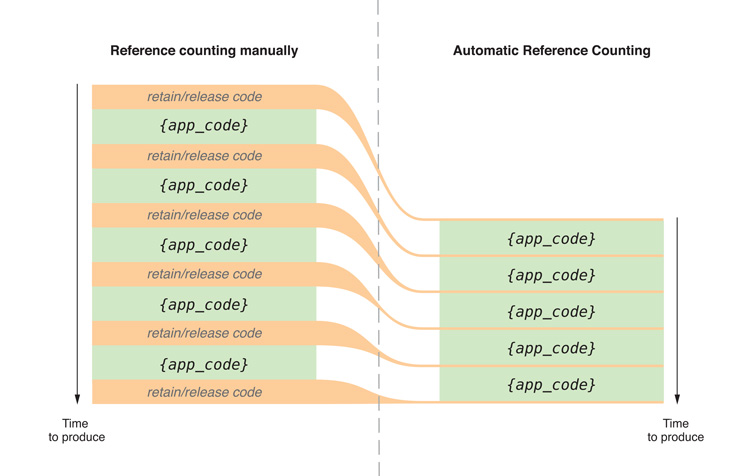
\includegraphics[scale=0.50]{immagini/ARC.jpg}
            \vspace{0.8cm}
            \caption{\textit{Confronto tra MMC ed ARC relativo al tempo di creazione dei cicli di retain-release degli oggetti}}
    \end{figure}
Il comportamento di ARC è però differente tra i due linguaggi:\\
In Swift il supporto è completo rispetto ai percorsi di codice procedurali ed \textit{object- oriented}; Objective-C invece supporta ARC solamente nell'utilizzo delle API Cocoa ed il codice object-oriented; questo significa che sarà ancora compito del programmatore gestire la memoria quando si utilizzano API come Core Graphics e altre di basso livello disponibili in iOS, creando il rischio di \textit{memory-leaks}.
\section{Performance}
Tester indipendenti hanno confrontato le performance dei due linguaggi su strutture dati standard: Array/NSArray e Dictionary/NSDictionary.\\\\
L'approccio utilizzato prevede la preinizializzazione delle strutture dati con un numero fisso di elementi; è stata effettuata solamente una operazione sulla struttura dati, quindi è stata creata una nuova struttura con un nuovo stato iniziale ed è stata eseguita nuovamente l'operazione.\\\\ Sono stati considerati 500 stati differenti per ogni struttura dati, e le performance sono state calcolate su 10 iterazioni.\\\\L'asse delle ascisse mostra il numero di elementi nella struttura dati, l'asse delle ordinate il tempo medio di esecuzione dell'operazione.
\subsubsection{Aggiunta di un elemento ad un array}
\begin{figure}[H]
      \centering
      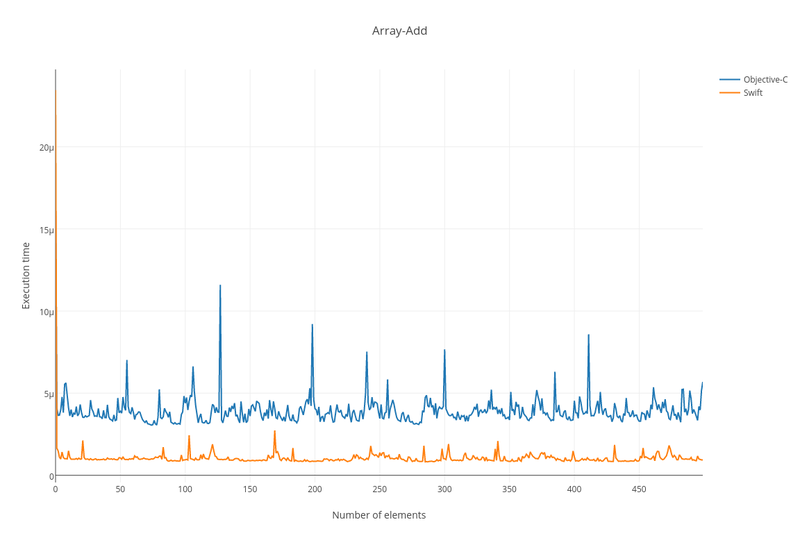
\includegraphics[scale=0.50]{immagini/array_add.png}
            \vspace{0.8cm}
            \caption{\textit{Complessità: costante per entrambi i linguaggi. L'aggiunta del primo elemento all'array dinamico in Swift è quattro volte più lento rispetto ad Objective-C.
Per gli array contenenti già elementi l'operazione in Swift è più veloce di due volte rispetto ad Objective-C}}
\end{figure}
\subsubsection{Rimozione di un elemento in un array}
\begin{figure}[H]
      \centering
      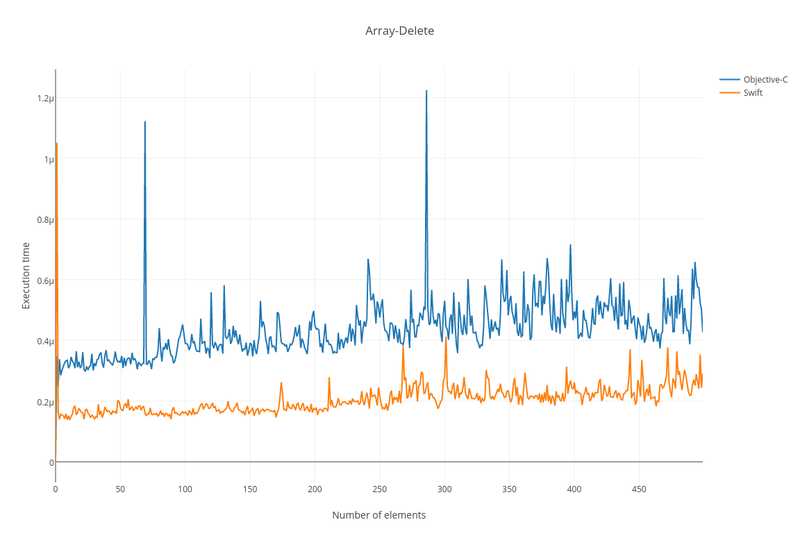
\includegraphics[scale=0.50]{immagini/array_delete.png}
            \vspace{0.8cm}
            \caption{\textit{Complessità: lineare per Swift, lineare inizialmente per poi passare a tempo costante per Objective-C}}
\end{figure}
\subsubsection{Lettura di un elemento in un array}
\begin{figure}[H]
      \centering
      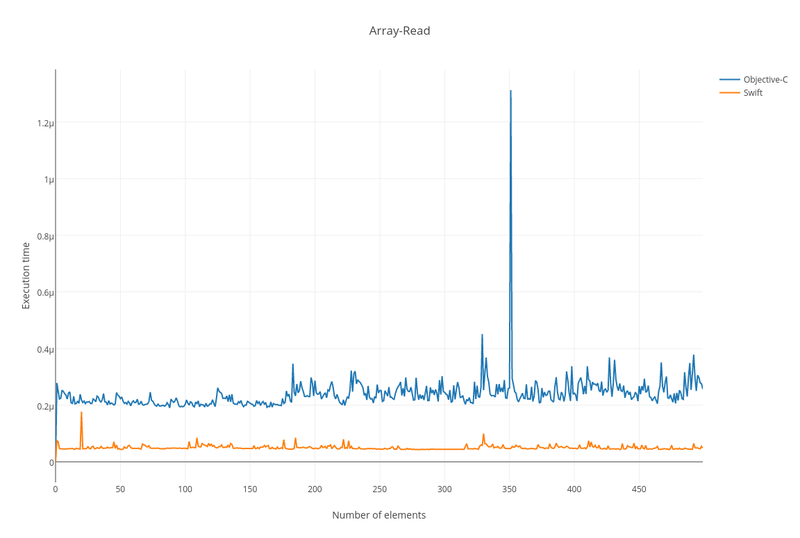
\includegraphics[scale=0.50]{immagini/array_read.png}
            \vspace{0.8cm}
            \caption{\textit{Complessità: costante per entrambi i linguaggi. Swift risulta dalle 4 alle 6 volte più rapido}}
\end{figure}
\subsubsection{Ricerca di un elemento in un array}
\begin{figure}[H]
      \centering
      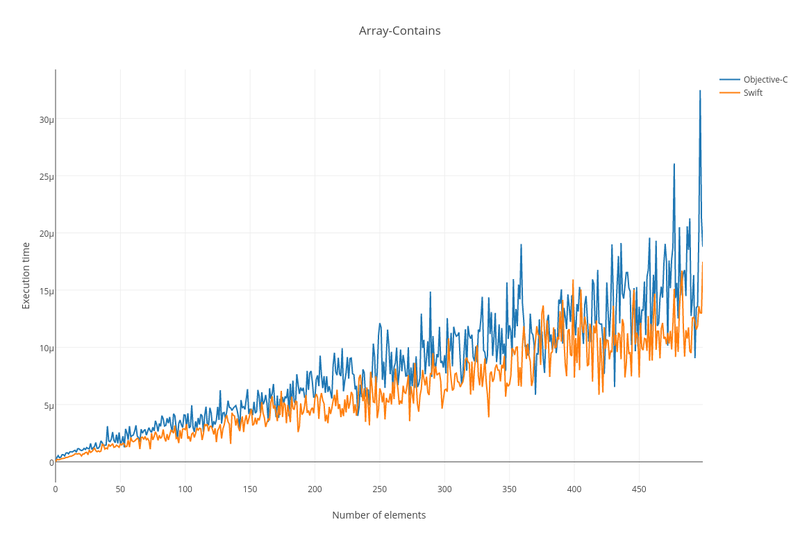
\includegraphics[scale=0.50]{immagini/array_contains.png}
            \vspace{0.8cm}
            \caption{\textit{Complessità: lineare per entrambi i linguaggi. I risultati per questa operazione vedono Swift leggermente più veloce}}
\end{figure}
\subsubsection{Aggiornamento di un elemento in un array}
\begin{figure}[H]
      \centering
      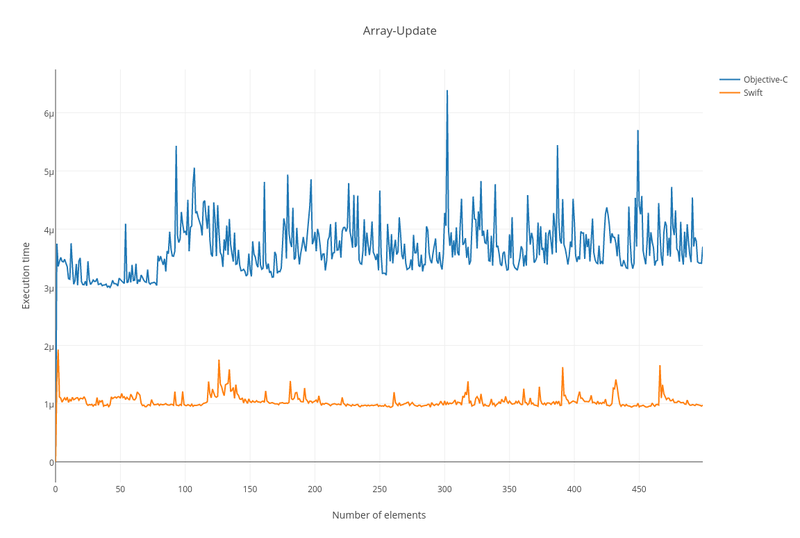
\includegraphics[scale=0.50]{immagini/array_update.png}
            \vspace{0.8cm}
            \caption{\textit{Complessità: costante per Swift, lineare inizialmente per per poi passare a tempo costante per Objective-C. Swift risulta dalle 3 alle 4 volte più veloce}}
\end{figure}
\subsubsection{Aggiunta di un elemento ad un dizionario}
\begin{figure}[H]
      \centering
      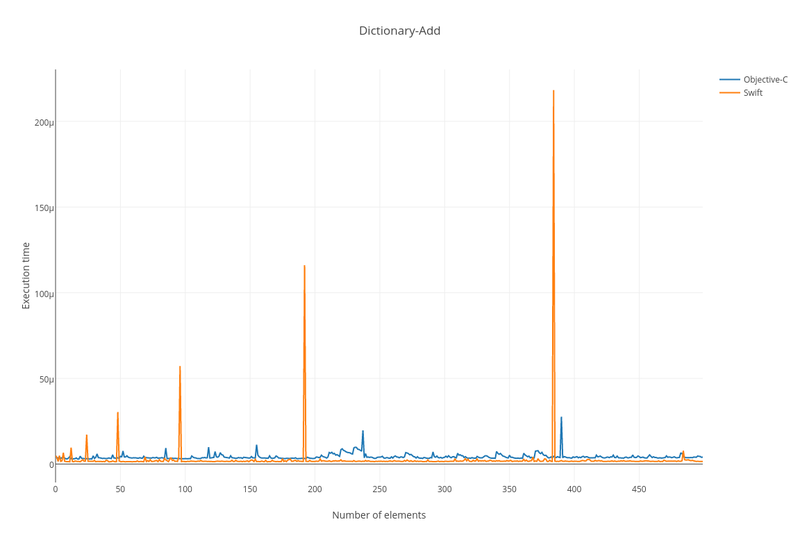
\includegraphics[scale=0.50]{immagini/dictionary_add.png}
            \vspace{0.8cm}
            \caption{\textit{Complessità: costante per entrambi; si possono notare dei picchi regolari nel tempo di esecuzione, spiegabili con l'allocazione di memoria per i nuovi elementi, in quanto il dizionario aumenta di 2 volte e non linearmente; Swift risulta dalle 2 alle 3 volte più veloce.}}
\end{figure} 
\subsubsection{Ricerca di un elemento in un dizionario}
\begin{figure}[H]
      \centering
      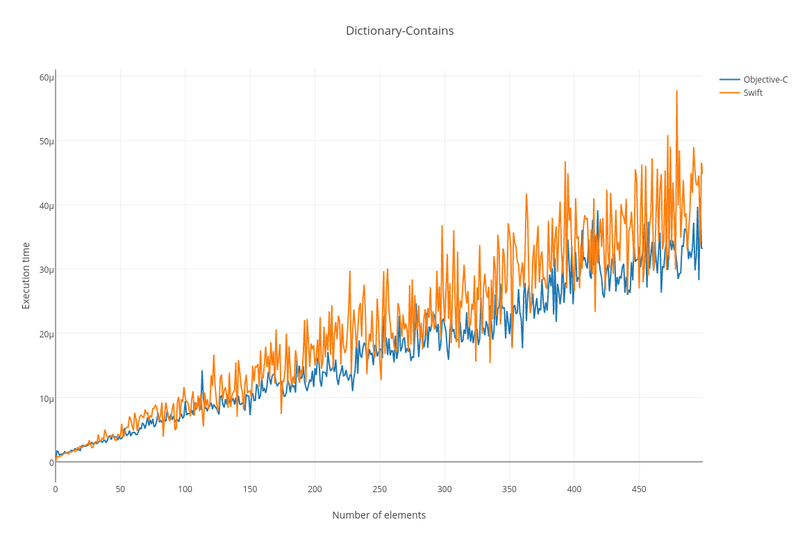
\includegraphics[scale=0.50]{immagini/dictionary_contains.png}
            \vspace{0.8cm}
            \caption{\textit{Complessità: lineare per entrambi i linguaggi; Swift risulta avere performance leggermente inferiori.}}
\end{figure}
\subsubsection{Rimozione di un elemento da un dizionario}
\begin{figure}[H]
      \centering
      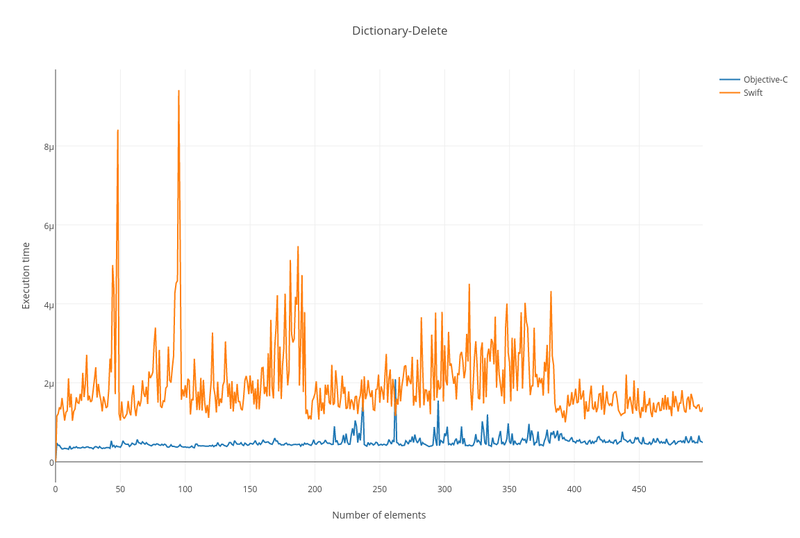
\includegraphics[scale=0.50]{immagini/dictionary_delete.png}
            \vspace{0.8cm}
            \caption{\textit{Complessità: costante per entrambi i linguaggi; Objective-C risulta dalle 3 alle 4 volte più veloce in questa operazione; Swift produce una curva con andamento ondulatorio, correlata al cambiamento dinamico della dimensione dell'array.}}
\end{figure}
\subsubsection{Lettura di un elemento da un dizionario}
\begin{figure}[H]
      \centering
      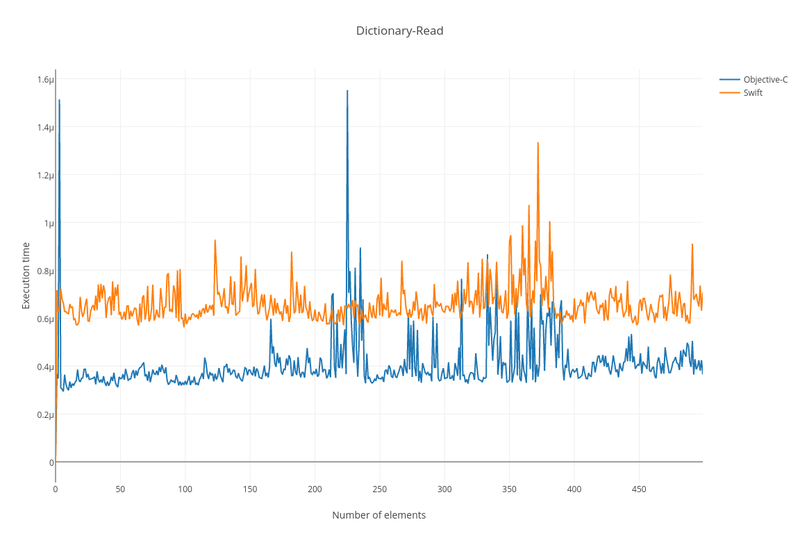
\includegraphics[scale=0.50]{immagini/dictionary_read.png}
            \vspace{0.8cm}
            \caption{\textit{Complessità: costante per entrambi i linguaggi; Objective-C risulta due volte più rapido.}}
\end{figure}
\subsubsection{Aggiornamento di un elemento di un dizionario}
\begin{figure}[H]
      \centering
      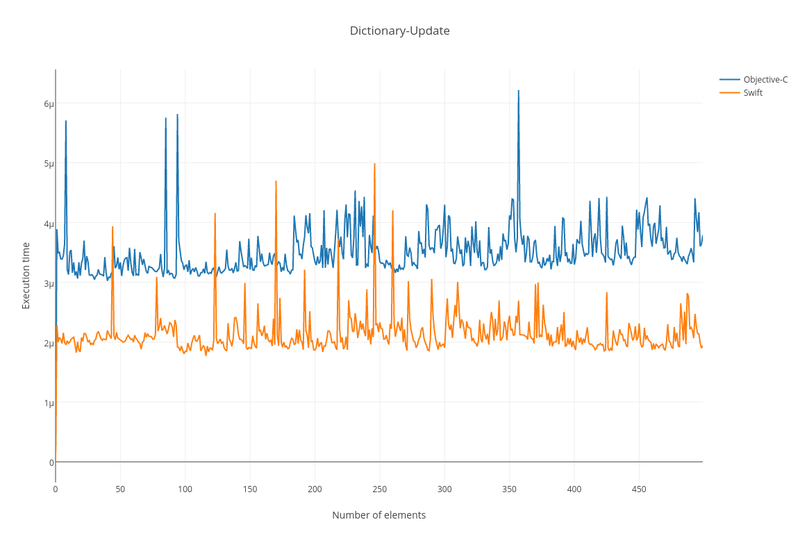
\includegraphics[scale=0.50]{immagini/dictionary_update.png}
            \vspace{0.8cm}
            \caption{\textit{Complessità: costante per Swift, lineare per Objective-C. Swift risulta 2 volte più rapido.}}
\end{figure}
\subsubsection{Conclusioni sulle performance}
Le operazioni sugli Array sono dalle due alle quattro volte più performanti in rispetto a quelle effettuate sugli NSArray; per migliorare le prestazioni si dovrebbero preinizializzare le strutture dati con il numero di elementi massimo conosciuto in anticipo.\\\\Tutte le operazioni tranne la ricerca (contains) vengono eseguite in tempo costante; nonostante Swift gestisca le operazioni di inserzione in un Dizionario e in un Set in maniera più efficiente, le altre operazioni soffrono in prestazioni rispetto ad Objective-C.\\
\\Gli Array risultano la struttura dati da preferire in Swift per tutte le operazioni (eccetto la ricerca) se si ha un gran numero di elementi; in questo caso un Set è preferibile.\\\\
Come si può notare, i grafici delle funzioni risultano particolari per un array in stile C, questo perché a livello implementativo non è un vero array C: Objective-C utilizza un complesso insieme di strutture dati che non sono Array nativi ma che espongono funzionalità da tale.
    
    
    
    


